\chapter{Conclusiones}

\section{Resultados}
En la figura \ref{tc-tests}, se puede ver la distribución de los casos de prueba
según el tipo de evaluación realizado, puede apreciarse que las pruebas
funcionales ocupan mas de la mitad de la totalidad de casos de prueba en el
proyecto, mientras que los casos de prueba negativos, y de aceptación, están más
próximos al 10\%.

\begin{figure}
\centering
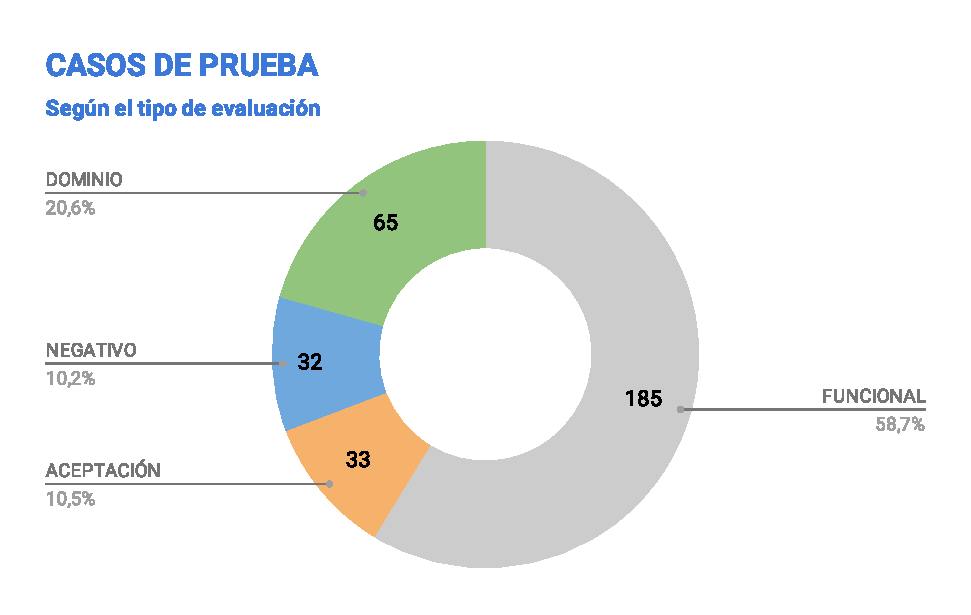
\includegraphics[width=1.0\textwidth]{graphics/tc-tests.eps}
\caption{Casos de Prueba según el tipo de evaluación realizada.}
\label{tc-tests}
\end{figure}

En la figura \ref{tc-type}, se puede ver la distribución de los casos de prueba
según el tipo de acción que se realiza en el sistema, es decir, si son casos
que afectan la interfaz de usuario, si mas bien son funciones de validación, o
si realizan alguna petición al servidor, sea esta de lectura o escritura.

Puede apreciarse igualmente que la mayor parte de los casos de prueba están
orientados a evaluar el comportamiento de la interfaz de usuario, mientras que
en un 25\% aproximadamente se evalúan funcionalidades que se comunican con el
servidor.

\begin{figure}
\centering
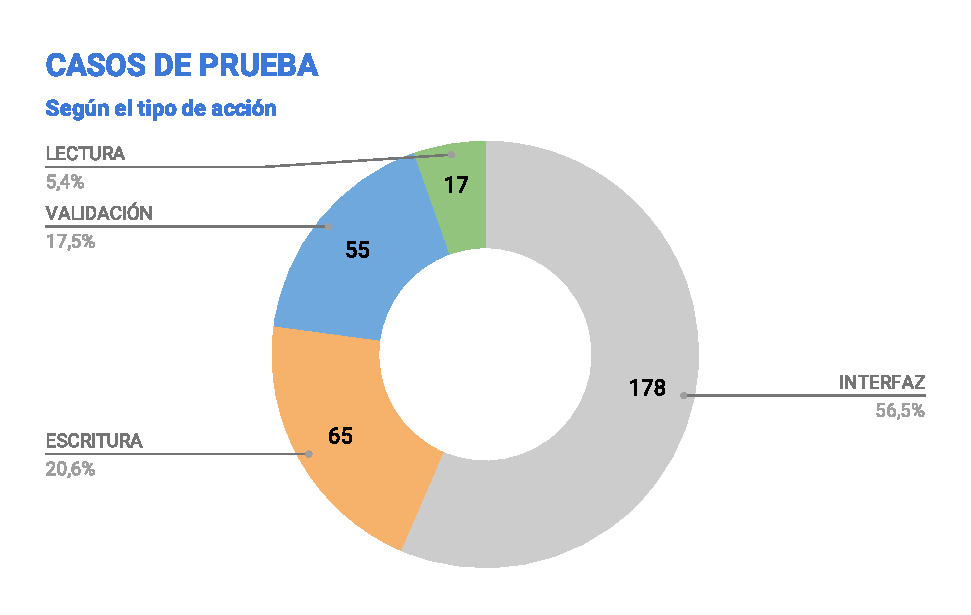
\includegraphics[width=1.0\textwidth]{graphics/tc-type.eps}
\caption{Casos de Prueba según el tipo de acción a evaluar.}
\label{tc-type}
\end{figure}

En las figuras \ref{results-tests} y \ref{results-type}, se condensan los
resultados obtenidos de la ejecución de los casos de prueba, en los cuales
únicamente fallaron 2 casos de prueba, ambos relacionados a un mismo formulario,
como puede verse en el reporte de error adjunto, y debido al fallo de estos
también se bloquearon dos casos de prueba.

\begin{figure}
\centering
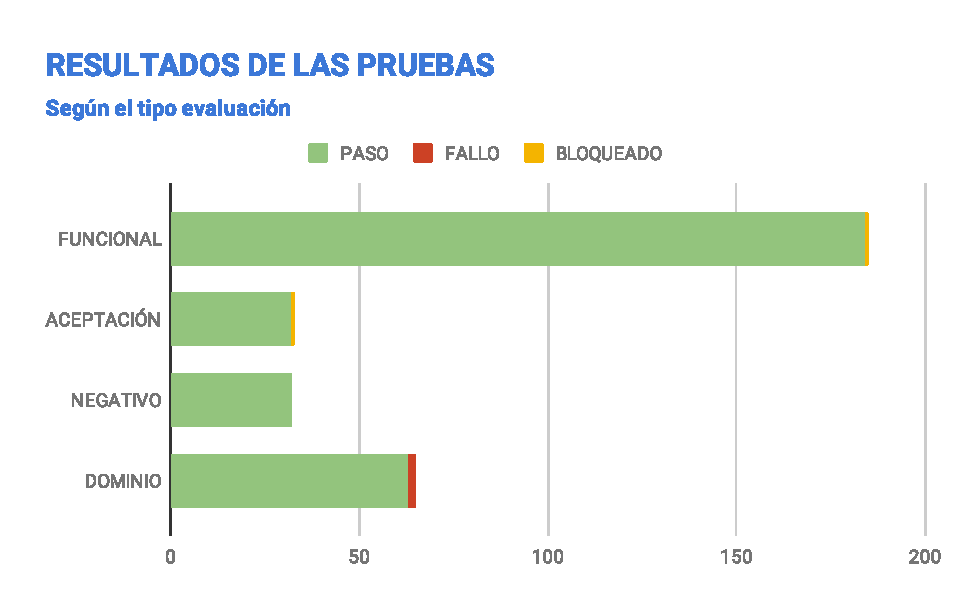
\includegraphics[width=1.0\textwidth]{graphics/results-tests.eps}
\caption{Resultados de las pruebas clasificadas por tipo de evaluación.}
\label{results-tests}
\end{figure}

\begin{figure}
\centering
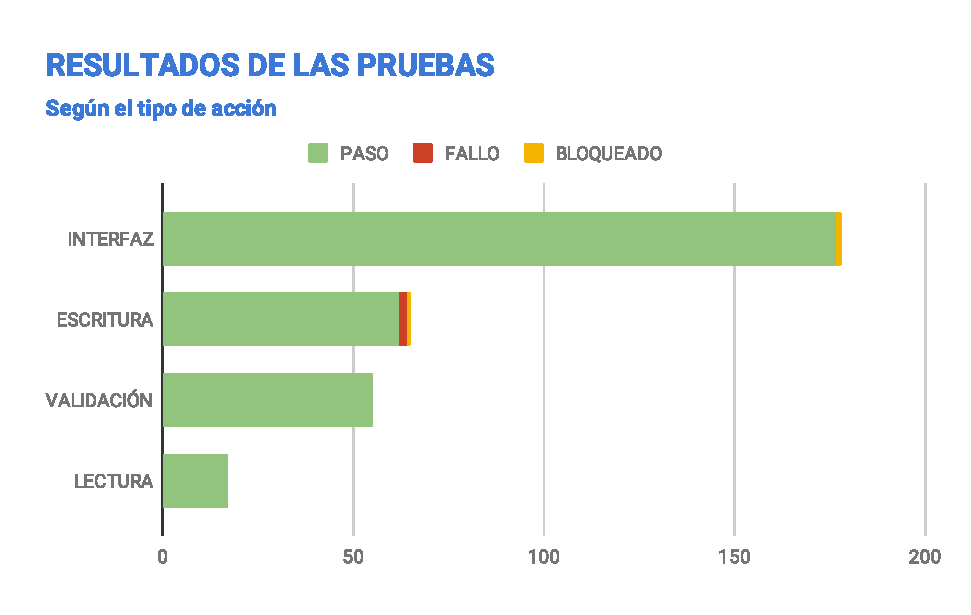
\includegraphics[width=1.0\textwidth]{graphics/results-type.eps}
\caption{Resultados de las pruebas clasificadas por tipo de acción a evaluar.}
\label{results-type}
\end{figure}

\section{Conclusiones}
Presentados los resultados de la ejecución de las pruebas, vemos que de los 315
casos de pruebas únicamente existes 2 bloqueados, y dos fallidos. Por ende se
tiene 98.74\% de casos de prueba exitosos, lo que lleva a concluir que los
atributos de calidad esperados del sistema están cubiertos por completo.

